\section{Marco Teórico}

\subsection{Definición y Partes del Contactor}

Un contactor es un interruptor accionado electromagnéticamente, diseñado para establecer o interrumpir corrientes en condiciones normales y ocasionales~\cite{wikipedia}. En la figura~\ref{fig:contactor} se muestra el aspecto externo de un contactor industrial típico, mientras que en la figura~\ref{fig:despiece_contactor} se detallan sus componentes internos y despiece.

\begin{figure}[htbp]
    \centering
    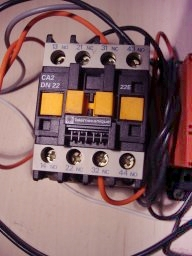
\includegraphics[width=0.45\textwidth]{figures/contactor.jpg}
    \caption{Contactor electromagnético industrial típico.}
    \label{fig:contactor}
\end{figure}

Sus partes fundamentales son:

\begin{itemize}
    \item \textbf{Bobina (circuito de magnetización):} Alimentada con tensión alterna o continua, genera la fuerza magnetomotriz que acciona el circuito magnético.
    \item \textbf{Núcleo magnético (estacionario):} Elemento ferromagnético fijo, generalmente laminado para reducir pérdidas por corrientes parásitas.
    \item \textbf{Armadura o martillo (móvil):} Parte móvil del circuito magnético que se desplaza al ser atraída por el núcleo cuando la bobina se energiza.
    \item \textbf{Contactos principales:} Conducen la corriente de servicio en condiciones normales.
    \item \textbf{Contactos auxiliares:} Utilizados en circuitos de control y señalización.
\end{itemize}

\begin{figure}[htbp]
    \centering
    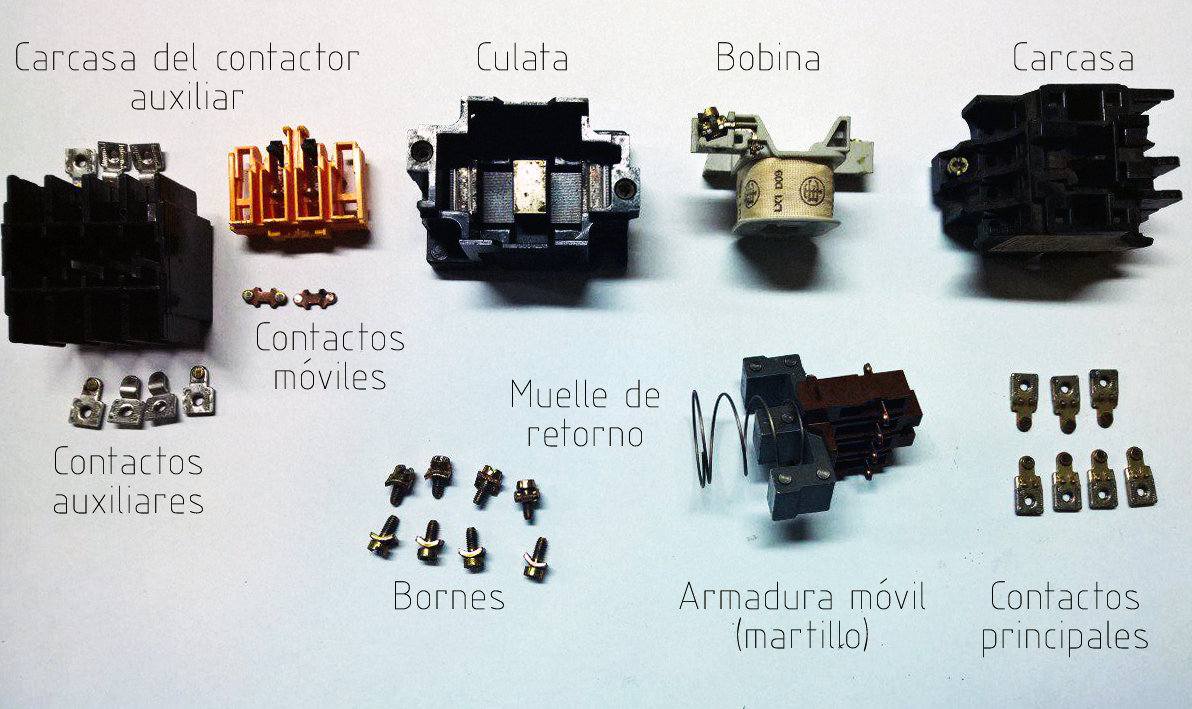
\includegraphics[width=0.7\textwidth]{figures/despiece_contactor.jpg}
    \caption{Despiece y partes constitutivas internas de un contactor electromagnético.}
    \label{fig:despiece_contactor}
\end{figure}

\subsection{Estados del Circuito Magnético}

El circuito magnético del contactor presenta dos estados bien diferenciados:

\begin{enumerate}
    \item \textbf{Reposo:} La bobina no está energizada. Existe un entrehierro grande entre el núcleo y la armadura, por lo que la reluctancia del circuito magnético es máxima.
    \item \textbf{Energizado o activado:} La bobina está energizada y la armadura es atraída contra el núcleo. El entrehierro se reduce al mínimo, la reluctancia disminuye y el flujo magnético se establece eficientemente.
\end{enumerate}

La corriente que circula por la bobina difiere significativamente entre ambos estados: en el momento de la activación se presenta la \textit{corriente de llamada}, que puede alcanzar de 6 a 10 veces la corriente de mantenimiento, debido a que la impedancia de la bobina es inicialmente baja por el gran entrehierro.

\subsection{Espiras de Sombra (Anillos Conductores)}

Las espiras de sombra son anillos de cobre o latón colocados en una porción de las columnas del núcleo magnético. Su función es generar un desfase en el flujo magnético de la zona sombreada respecto a la no sombreada, evitando que el par magnético se anule en los cruces por cero de la corriente alterna. Esto elimina la vibración y el zumbido característico del contactor durante su operación.

\subsection{Entrehierro Permanente}

El entrehierro permanente es una separación deliberada entre el núcleo y la armadura, impuesta por la desigualdad en las longitudes de las columnas del núcleo magnético. Su propósito es evitar el fenómeno de \textit{remanencia magnética}: si no existiera este entrehierro, la armadura podría quedar adherida al núcleo por el magnetismo remanente incluso después de desenergizar la bobina, impidiendo la apertura de los contactos.

\subsection{Corriente de Llamada y Corriente de Mantenimiento}

\begin{itemize}
    \item \textbf{Corriente de llamada ($I_{\text{llamada}}$):} Corriente transitoria que circula por la bobina en el instante de la energización, cuando el entrehierro es máximo. Su magnitud es de 6 a 10 veces la corriente de mantenimiento.
    \item \textbf{Corriente de mantenimiento ($I_{\text{mant}}$):} Corriente en régimen permanente que circula por la bobina una vez que la armadura ha cerrado el circuito magnético.
\end{itemize}

La tensión de mantenimiento es la tensión mínima requerida en la bobina para mantener la armadura en la posición cerrada.

\subsection{Normas Aplicables}

Los contactores se fabrican conforme a normas internacionales:

\begin{itemize}
    \item \textbf{IEC 60947:} Norma internacional para aparamenta de baja tensión.
    \item \textbf{UL 508:} Estándar estadounidense para equipos de control industrial.
    \item \textbf{NEMA ICS:} Norma norteamericana para controladores industriales.
\end{itemize}

Estas normas definen parámetros como corriente de empleo, corriente térmica nominal, tensión de servicio, potencia nominal, clase de servicio y categorías de servicio.

\subsection{Parámetros Característicos}

\begin{itemize}
    \item Corriente de empleo o de servicio nominal ($I_e$)
    \item Corriente térmica nominal ($I_{th}$)
    \item Tensión de servicio nominal ($U_e$)
    \item Potencia de servicio nominal
    \item Tipo de cerramiento
    \item Clase de servicio
    \item Categorías de servicio (AC-1, AC-3, AC-4, etc.)
\end{itemize}
